\chapter{Evaluation de l'efficacité du Neurofeedback par la méta-analyse} \label{chapitre-2}

\section*{Introduction}
Les méta-analyses ont pour but de combiner les données de plusieurs études visant à démontrer l'efficacité d'un traitement. Cette méthode est
particulièrement intéressante lorsque les études comportent un faible nombre de sujets, comme c'est notamment le cas dans la plupart de celles sur 
le \gls{nfb} appliqué aux enfants \gls{tdah}. 

Les différentes étapes à suivre pour réaliser une méta-analyse sont détaillées dans ce chapitre et résumées en Figure~\ref{Figure:pipeline_meta_analyse}.
Ces étapes sont ensuite appliquées à la réplication et à la mise à jour d'une récente méta-analyse sur le \gls{nfb} appliqué aux enfants \gls{tdah} :
celle de \citet{Cortese2016}, dont certains résultats ont été débattus par la communauté scientifique \citep{Micoulaud2016}. Ainsi, cette analyse a pour but
de mettre en évidence l'éventuel impact de certains choix de \citet{Cortese2016} sur ses conclusions quant à l'efficacité du \gls{nfb} et de mettre à jour
ces résultats en incluant de nouvelles études. 

A travers le travail présenté ici, la performance du \gls{nfb} sur les enfants \gls{tdah} est alors évaluée et la revue de littérature
qui a été menée a permis de s'imprégner des problématiques de cette technique.

\clearpage

\section{Principe d'une méta-analyse} \label{methods}

Les différentes étapes pour réaliser une méta-analyse sont décrites dans cette partie. Bien qu'il existe des logiciels permettant de réaliser une
méta-analyse, ces étapes ont été implémentées en Python par souci de transparence et de reproductibilité dont le code source est disponible sur un 
dépôt GitHub \citep{Bussalb2019clinical} avec sa documentation associée générée par Sphinx (version 1.5.6.).

\subsection{Buts d'une méta-analyse}

Les méta-analyses rassemblent les résultats de plusieurs études, satisfaisant des critères d'inclusion préalablement établis, dans le but d'analyser
sur un plus grand nombre de sujets provenant de populations différentes, l'efficacité d'un traitement. Alors qu'avant les années 1990 les revues narratives
(\textit{narrative reviews} en anglais) étaient le plus couramment utilisées pour cette tâche, elles ont perdu leur popularité au profit des méta-analyses.
En effet, les revues narratives souffrent de la subjectivité des auteurs qui choisissent notamment le poids à donner à telle ou telle étude : alors que certains
vont donner plus d'importance aux études incluant de nombreux sujets, d'autres vont favoriser les études qu'ils jugent de bonne qualité. La méta-analyse permet 
de réduire cette subjectivité en utilisant par exemple des critères mathématiques définis à l'avance pour calculer le poids à attribuer à chaque étude incluse
\citep{Borenstein2009}.

Réaliser une méta-analyse permet de confronter les résultats de toute étude incluse à ceux des autres études intégrées dans l'analyse : l'efficacité (mesurée par 
une valeur standardisée appelée taille d'effet ou \gls{es} en anglais) est-elle constante parmi l'ensemble des études sélectionnées ? 
Auquel cas, l'\gls{es} doit être calculé précisément, sinon on cherche à quantifier à quel point l'efficacité entre les études varie.

\subsection{Choix du modèle}

La première étape consiste à choisir le modèle statistique de la méta-analyse. La plupart des méta-analyses sont basées sur l'un des deux modèles 
suivants qui reposent sur des hypothèses scientifiques différentes \citep{Borenstein2009} :
\renewcommand{\labelitemi}{$\bullet$}
\begin{itemize}
\item le modèle à effet fixe (\textit{fixed-effect model} en anglais),
\item le modèle à effets aléatoires (\textit{random-effects model} en anglais).
\end{itemize}

Dans le cas du modèle à effet fixe, il est supposé qu'il existe un \gls{es} réel (\textit{true} \gls{es} en anglais), c'est à dire l'\gls{es} qui serait
observé avec un nombre de sujets infiniment grand, qui serait le même pour l'ensemble des études incluses dans la méta-analyse. Les différences entre
les \gls{es} observés pour chaque étude sont dues à des erreurs d'échantillonnage. Au contraire, dans le cas du modèle à effets aléatoires, 
l'\gls{es} réel peut varier entre les études. Cette variabilité s'explique non seulement par des erreurs d'échantillonnage mais aussi par 
les différentes conceptions des études et/ou par les différences entre les sujets inclus.

L'hypothèse nulle testée lors de la méta-analyse est différente selon le modèle choisi :
\begin{itemize}
\item pour le modèle à effet fixe : 
\textit{$H_{0}$ : le traitement n'a auncun effet dans chaque étude},
\item pour le modèle à effets aléatoires : 
\textit{$H_{0}$ : l'effet moyen du traitement est nul}.
\end{itemize}

Le modèle à effets aléatoires est souvent plus approprié du fait de la variabilité des études. En effet, même si les études incluses dans la méta-analyse 
répondent toutes aux critères d'inclusion fixés au préalable, rien ne peut généralement permettre de supposer que ces études sont identiques et qu'elles 
partagent donc toutes le même \gls{es} réel. Le modèle à effet fixe est ainsi rarement utilisé, on peut cependant y avoir recours lorsque le nombre d'études incluses 
est très petit. Au sein du domaine du \gls{nfb} appliqué aux enfants \gls{tdah}, les méta-analyses suivent le modèle à effets aléatoires 
\citep{Cortese2016, Micoulaud2014}, c'est donc ce modèle que nous choisissons également.

\subsection{Calcul de la taille d'effet}

Une fois le modèle choisi, l'étape suivante est de quantifier l'efficacité de chaque étude incluse dans la méta-analyse en calculant son \gls{es}. 
Il existe différents \gls{es} \citep{Borenstein2009} :
\renewcommand{\labelitemi}{$\bullet$}
\renewcommand{\labelitemii}{$\cdot$}
\begin{itemize}
\item \gls{es} basés sur des \emph{moyennes} :
\begin{itemize}
    \item la différence moyenne non standardisée (\textit{unstandardized mean difference} en anglais), D :
		    \begin{equation}
        \label{eq:metareview_unstandardized_mean_difference}
        \text{D} = \bar{X}_{1} - \bar{X}_{1},
        \end{equation} 
		avec $\bar{X}_{1}$ et $\bar{X}_{2}$ les moyennes de deux groupes indépendants, ou du même groupe à pré- et à post-test,
    \item la différence moyenne standardisée (\textit{standardized mean difference} en anglais), d :
		    \begin{equation}
        \label{eq:metareview_standardized_mean_difference}
        \text{d} = \frac{\bar{X}_{1} - \bar{X}_{2}}{\sqrt{\frac{(n_1 - 1)S_1^2 + (n_2 - 1)S_2^2} {n_1 + n_2 - 2}}},
        \end{equation} 
		avec $n_{1}$ et $n_{2}$ le nombre de sujets dans les groupes 1 et 2, et $S_{1}$ et $S_{2}$ les écarts types des deux groupes. Le dénominateur
		correspond à l'écart type intra-groupes calculé à travers les deux groupes.
\end{itemize}
\item \gls{es} basés sur des \emph{données binaires} :
\begin{itemize}
    \item le taux de risque (\textit{risk ratio} en anglais), RR :
				\begin{equation}
        \label{eq:metareview_risk_ratio}
        \text{RR} = \frac{ \text{A} / n_1 } { \text{C} / n_2 },
        \end{equation} 
		avec A et C est le nombre d'évènements observés (par exemple présence d'un effet secondaire) respectivement dans les groupes 1 et 2,
    \item le taux de chance (\textit{odds ratio} en anglais), OR :
				\begin{equation}
        \label{eq:metareview_odds_ratio}
        \text{OR} = \frac{ \text{AD} } { \text{BC} },
        \end{equation} 		
		avec D et B le nombre de non évènements observés (par exemple absence d'un effet secondaire) respectivement dans les groupes 2 et 1,
		\item la différence de risque (\textit{risk difference} en anglais), RD :
				\begin{equation}
        \label{eq:metareview_risk_difference}
        \text{RD} = \frac{ \text{A} } { n_1 } - \frac{ \text{C} } { n_2 }.
        \end{equation}
\end{itemize}
\end{itemize}

Etant donné que les données que nous allons utiliser pour la réplication et la mise à jour de \citet{Cortese2016} sont les moyennes des 
scores cliniques obtenus par les sujets sur des échelles évaluant les symptômes du \gls{tdah} avant le traitement (pré-test) et 
après le traitement (post-test) et leur écart-type, nous nous concentrons sur 
les \gls{es} basés sur des moyennes. Par ailleurs, les échelles cliniques variant 
d'une étude à l'autre, les moyennes ne sont pas comparables : il faut donc standardiser l'\gls{es}. 
Ainsi, nous allons utiliser la différence moyenne standardisée d \citep{Cortese2016, Micoulaud2014}.

Enfin, lorsqu'un groupe contrôle est disponible, on peut calculer l'\gls{es}-inter-groupes (\textit{between}-\gls{es}) comme défini par \citet{Morris2008}.
Cet \gls{es} est utilisé par \citet{Cortese2016, Micoulaud2014} et implémenté dans \citet{Bussalb2019clinical} :
\begin{equation}
\label{eq:metareview_effect_size_between}
\text{ES-inter-groupes} = c_p \left(\frac{(M_{\text{post},T} - M_{\text{pre},T}) - (M_{\text{post},C} - M_{\text{pre},C}) }{\sigma_{\text{pre}}} \right).
\end{equation} 
L'\gls{es}-inter-groupes est équivalent au z-score d'une distribution normale. Il correspond à la différence entre la moyenne à post-test et à pré-test 
dans le groupe qui reçoit le traitement ($M_{\text{pre},T}$, $M_{\text{post},T}$) moins la différence entre la moyenne du score à post-test et à pré-test 
dans le groupe contrôle ($M_{\text{pre},C}$, $M_{\text{post},C}$), divisée par la \textit{pooled} standard deviation à pré-test ($\sigma_{\text{pre}}$) :
\begin{equation}
\label{eq:stats_metareview_std_pre}
\sigma_{\text{pre}} = \sqrt{\frac{(n_T - 1)\sigma_{\text{pre},T}^2 + (n_C - 1)\sigma_{\text{pre},C}^2} {n_T + n_C - 2}},
\end{equation}
où $\sigma_{t,G}$ correspond à l'écart-type du groupe $G$ à pré-test and $n_G$ indique le nombre de sujets dans chaque groupe ; 
$c_p$ est un bias d'ajustement utilisé pour les petites études (c'est à dire pour lesquelles $n_T + n_C - 2 < 10$) : 
\begin{equation}
\label{eq:metareview_correction_factor}
c_p =  1 - \frac{3} {4(n_T + n_C - 2) - 1}.
\end{equation} 

\subsection{Calcul de la précision de chaque taille d'effet}

Le terme précision englobe trois valeurs statistiques liées les unes aux autres : la variance, l'erreur standard, et l'intervalle de confiance.
Ces trois facteurs de précision définissent un intervalle de valeurs probables pour l'\gls{es} réel. 

Tout d'abord, la variance de chaque \gls{es}-inter-groupes est calculée \citep{Morris2008}:
\begin{equation}
\label{eq:metareview_variance_effect_size_between}
\sigma^2(\text{ES}) = c_p^2 \left (\frac{n_T + n_C - 2} {n_T + n_C - 4} \right ) \left  (\frac{2(1-r)(n_T + n_C)} {n_Tn_C} + \text{ES}^2 \right) - \text{ES}^2,
\end{equation}
où \gls{es} désigne l'\gls{es}-inter-groupes et $r$ la \textit{pooled} corrélation de Pearson intra-groupes \citep{James2013} :
\begin{equation}
\label{eq:metareview_within_group_pearson_correlation}
r = \frac{ \sum_{i=1}^{n} (\text{pre}_i - \mu_{\text{pre}})(\text{post}_i - \mu_{\text{post}}) } { \sqrt{ \sum_{i=1}^{n} (\text{pre}_i - 
\mu_{\text{pre}})^2} \sqrt{\sum_{i=1}^{n} (\text{post}_i - \mu_{\text{post}})^2} }, 
\end{equation}
où $n$ est le nombre de patients inclus dans une étude, $\text{pre}_i$, $\text{post}_i$ les valeurs de scores cliniques pour le sujet $i$ 
respectivement à pré- et post-test, et $\mu_{\text{pre}}$, $\mu_{\text{post}}$ les scores moyens calculés sur tous les sujets. 
Il s'agit d'une mesure de corrélation linéaire entre deux variables : une valeur de 1 signifie une corrélation positive entre ces variables,
une valeur de -1 une corrélation négative, et une valeur de 0 une absence de corrélation linéaire. 
Dans notre cas, cette corrélation étant inconnue et les données brutes n'étant pas disponibles, nous approximons la valeur de $r$ 
en accord avec \citet{Balk2012}, qui a trouvé qu'une valeur de 0.5 conduit à des résultats proches de ceux obtenus avec la véritable
valeur de la corrélation.

Une fois la variance obtenue, il est aisé de calculer l'\gls{et} (\textit{standard error} en anglais) de l'\gls{es}-inter-groupes 
\citep{Borenstein2009} :
\begin{equation}
\label{eq:metareview_standard_error_effect_size_between}
\text{ET} = \sqrt{\sigma^2(\text{ES})},
\end{equation}
où \gls{es} désigne l'\gls{es}-inter-groupes. Alors que la variance est intéressante pour les calculs statistiques, l'\gls{et} est quant à elle 
un index plus aisé à comprendre car elle est sur la même échelle que l'\gls{es}.

Enfin, si l'\gls{es}-inter-groupes suit une distribution normale, l'intervalle de confiance à 95\% peut être calculé \citep{Borenstein2009}.

La précision est affectée, dans une large mesure, par le nombre de sujets inclus dans l'étude : les échantillons plus grands mènent à des
estimations de \gls{es}-inter-groupes plus précises, c'est pourquoi un plus grand poids leur est attribué dans la méta-analyse.

\subsection{Calcul de l'effet total du traitement}

Afin d'obtenir l'estimation la plus précise possible de l'effet du traitement sur la population, une moyenne pondérée des \gls{es}-inter-groupes 
des études incluses est calculée.

Si le modèle à effet fixe est choisi, le poids $w_{\text{fixe}_k}$ assigné à chaque étude $k$ correspond à l'inverse de la variance de son 
\gls{es}-inter-groupes ($\sigma^2(\text{ES})$, la variance intra-étude) \citep{Borenstein2009} :
\begin{equation}
\label{eq:metareview_weight_fixed_study}
w_{\text{fixe}_k} = \frac{1}{\sigma^2(\text{ES}_k)}.
\end{equation} 

Dans notre cas nous employons le modèle à effets aléatoires, qui inclut également la variance inter-études $\tau^2$ conduisant à des 
poids ($w_{\text{aléatoires}_k} = w_k$) associés aux études différents.

Calculer la variance inter-études se fait en trois étapes décrites par les équations Eq.~(\ref{eq:metareview_Q}), Eq.~(\ref{eq:metareview_C}) 
et Eq.~(\ref{eq:metareview_Tau}) \citep{Borenstein2009} :
\begin{equation}
\label{eq:metareview_Q}
Q = \sum_{k=1}^{K} (w_{\text{fixe}_k} \text{ES}_k^2),
\end{equation}
\begin{equation}
\label{eq:metareview_C}
C = \sum_{k=1}^{K} w_{\text{fixe}_k} - \frac{ \sum_{k=1}^{K} (w_{\text{fixe}_k})^2 } { \sum_{k=1}^{K} w_{\text{fixe}_k} },
\end{equation}
avec $K$ le nombre total d'études incluses.
\begin{equation}
\label{eq:metareview_Tau}
\tau^2 = \frac{Q - \text{df}}{C},
\end{equation}
avec $\text{df} = K - 1$ le degré de liberté.

Le modèle à effets aléatoires prenant en compte les différences entre les études, les poids sont égaux à l'inverse de la somme entre la variance intra-étude
$\sigma^2(\text{ES}_k)$ et la variance inter-études $\tau^2$ \citep{Borenstein2009} :
\begin{equation}
\label{eq:metareview_weight_study}
w_k = \frac{1}{\sigma^2(\text{ES}_k) + \tau^2}.
\end{equation} 

Enfin, la moyenne pondérée des $K$ \gls{es}-inter-groupes est calculée pour obtenir l'\gls{est} comme décrit dans l' 
Eq.~(\ref{eq:metareview_summary_effect}) \citep{Borenstein2009}:
\begin{equation}
\label{eq:metareview_summary_effect}
\text{EST} = \frac{\sum_{k=1}^{K} w_k \text{ES}_k} {\sum_{k=1}^{K} w_k}.
\end{equation} 
Une fois l'\gls{est} obtenu, on peut calculer sa variance, son erreur type, son intervalle de confiance à 95\%, sa p-value, 
et $I^2$ qui estime l'hétérogénéité des \gls{es}-inter-groupes. 

Si la p-value calculée est inférieure à 0.05, alors il y a une différence statistiquement significative entre l'efficacité du traitement étudié 
et celle du groupe contrôle.

\subsection{Répresentation graphique des résultats d'une méta-analyse}

Afin de faciliter la lecture des résultats d'une méta-analyse, ceux-ci sont résumés dans un \textit{forest plot} \citep{Borenstein2009}. Les études incluses sont
en ordonnées et les \gls{es}-inter-groupes en abscisses. Chaque \gls{es}-inter-groupes est représenté par un carré dont la taille est proportionnelle
au poids $w_k$ attribué à l'étude $k$. Les intervalles de confiance à 95\% pour chaque \gls{es}-inter-groupes sont représentés. En bas du graphique, l'\gls{est}
est symbolisé par un diamant avec son intervalle de confiance à à 95\%. Une droite verticale d'équation $x = 0$ est tracée pour délimiter la
partie du graphique où les \gls{es} sont en faveur du traitement de celle où ils ne le sont pas.

Un autre graphique très utilisé dans la méta-analyse est le \textit{funnel plot} qui a pour but de détecter un éventuel biais de publication
lors de la sélection des études et une hétérogénéité parmi elles \citep{Sterne2011}. Il s'agit d'un nuage de points de la précision de chaque 
\gls{es}-inter-groupes en fonction des \gls{es}-inter-groupes. L'inverse de l'\gls{et} est couramment utilisé comme estimation de la précision et de la 
taille d'une étude et est placé sur un axe des abscisses inversé de façon à ce que les plus grandes études soient au sommet et que les plus petites se retrouvent 
dispersées en bas. En l'absence de biais et d'hétérogénéité entre les études, la répartition des points est seulement due à la variabilité de la taille des études : 
le graphique est symétrique. Le triangle centré sur \gls{est}, obtenu avec un modèle à effet fixe et s'étendant de 1.96 \gls{et} de chaque côté, 
inclut 95\% des études s'il n'y a pas de biais. Déterminer l'asymétrie d'un \textit{funnel plot} peut se faire visuellement mais aussi mathématiquement en utilisant, par exemple, le test d'\citet{Egger1997}. 
Il s'agit de régresser les \gls{es}-inter-groupes divisés par leur \gls{et} sur l'inverse des \gls{et}. Si l'intercept diffère significativement de 
0 (seuil de signifiance à 0.05), alors le \textit{funnel plot} est asymétrique.

L'ensemble des étapes pour réaliser une méta-analyse en suivant le modèle à effets aléatoires est résumé à la Figure~\ref{Figure:pipeline_meta_analyse}.

\begin{figure}[h!]
  \centering
	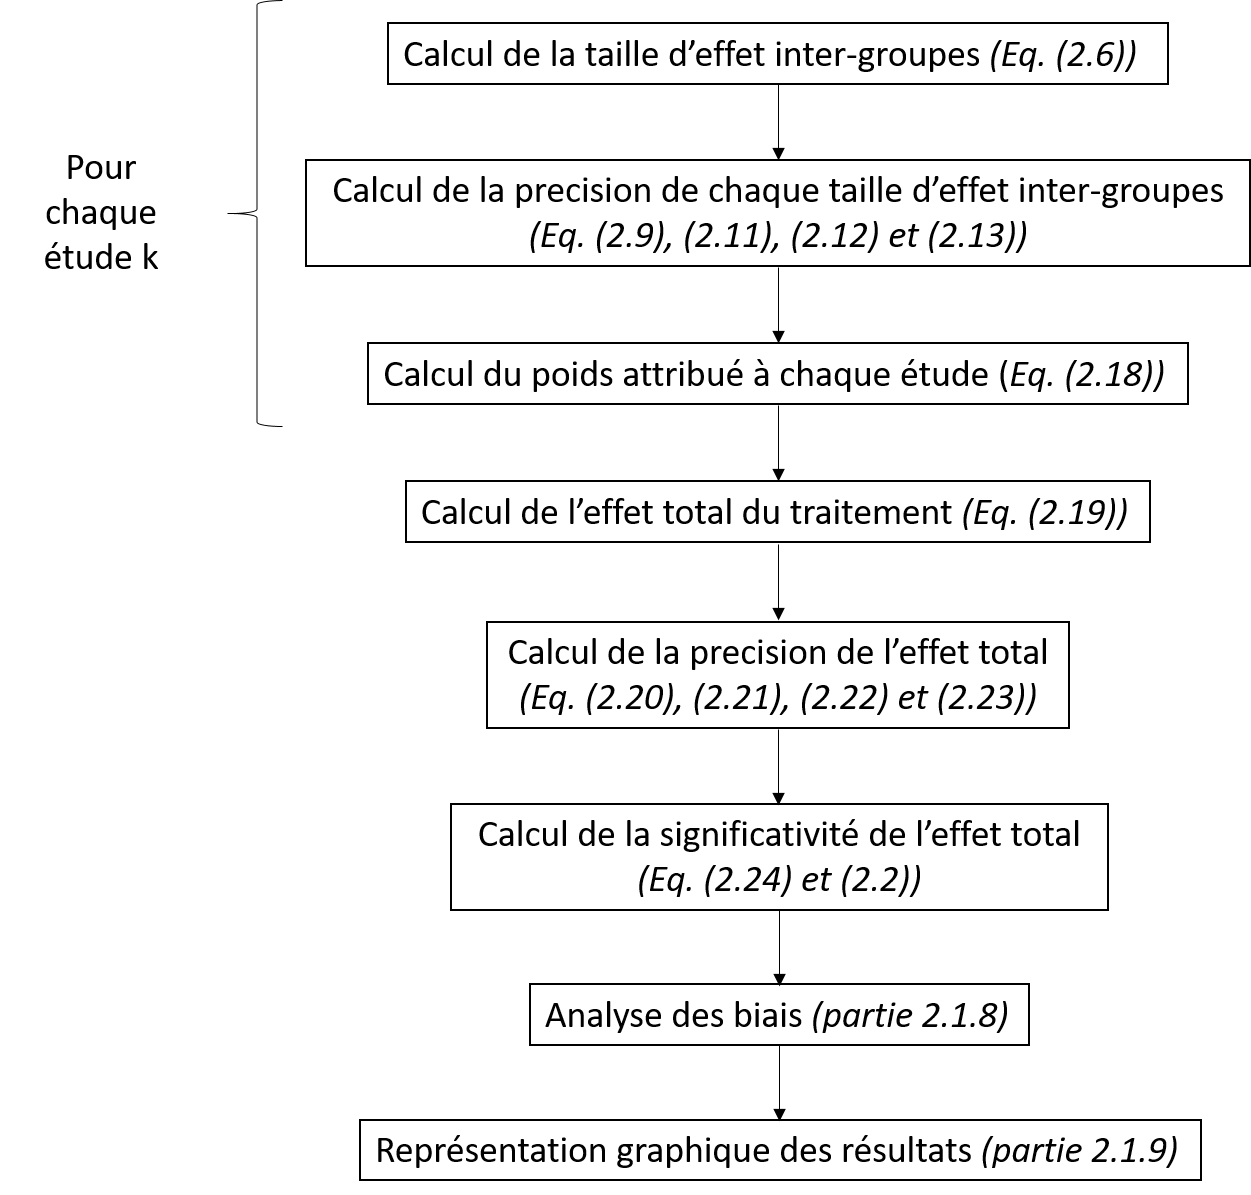
\includegraphics[width=1.0\linewidth]{figures/chapter-2/pipeline-perform-meta-analysis} 
  \caption{Résumé des étapes à suivre pour effectuer une méta-analyse dans le cadre d'un modèle à effets aléatoires.}
  \label{Figure:pipeline_meta_analyse}
\end{figure}

\section{Replication et mise à jour de la méta-analyse de Cortese et al., 2016} 

La méta-analyse de \citet{Cortese2016} a eu un fort impact dans la communauté du \gls{nfb}, du fait du nombre d'études incluses (13) et 
du soin apporté à la sélection de ces études. Cependant, quelques choix faits par les auteurs, comme le souligne \citet{Micoulaud2016}, méritent d'être explorés.
C'est pourquoi dans un premier temps, la méta-analyse de \citet{Cortese2016} est répliquée en modifiant les points débattus pour évaluer leur impact sur les
résultats. Ensuite, étant donné que la recherche dans le domaine du \gls{nfb} appliqué aux enfants \gls{tdah} est très active, de nouvelles études répondant au 
critère d'inclusion de \citet{Cortese2016} ont pu être publiées depuis cette méta-analyse. La mise à jour de ce genre d'analyse est importante
car plus des études y seront incluses, plus les résultats vont se stabiliser, c'est pourquoi nous allons relancer l'analyse avec les nouvelles études
satisfaisant les critères d'inclusion de \citet{Cortese2016}.

Dans un souci de transparence et pour faciliter la réplication de ce travail, ces deux analyses sont effectuées en utilisant le package Python 
(version de Python 3.6.1) dont le contenu est décrit en \ref{methods} \citep{Bussalb2019c}. Par conséquent, la première étape est d'évaluer la
fiabilité des résultats obtenus avec ce package.

\subsection{Evaluation des résultats obtenus avec le package Python}

Pour effectuer une méta-analyse, les auteurs utilisent en général le logiciel RevMan \citep{Revman, Cortese2016, Micoulaud2014}. Ici, les résultats 
obtenus avec le package Python vont être comparés à ceux donnés par la version 5.1 de RevMan, afin d'évaluer la précision du package. 

La première étape a été d'entrer dans un fichier .csv, pour chaque étude incluse, les moyennes des scores cliniques à pré-test et post-test avec leur écart-type utilisés 
par \citet{Cortese2016} pour calculer les \gls{es}-inter-groupes. Lorsqu'ils sont disponibles les scores cliniques évaluant l'inattention, l'hyperactivité 
et la totalité des symptômes sont extraits afin d'obtenir une valeur d'efficacité pour chacune de ces composantes. Par ailleurs, les scores donnés par les
parents (\gls{mprox}) mais aussi par les enseignants (\gls{pblind}) sont utilisés.

Une fois cette étape remplie, le package Python lit ce fichier et retourne l'\gls{est} ainsi que sa p-value associée qui permet de conclure quant à l'efficacité
du \gls{nfb} sur chaque composante. En accord avec les résultats de précédentes méta-analyses \citep{Sonuga-Barke2013, Micoulaud2014}, \citet{Cortese2016}
met en évidence un effet significativement favorable du \gls{nfb} lorsque son efficacité est calculée grâce aux évaluations des parents, mais aucune amélioration 
significative des symptômes n'est reportée par les enseignants. Ces résultats sont retrouvés lorsque l'analyse est effectuée par le programme Python, les valeurs
d'\gls{est} et leur p-value obtenues sont très proches voire égales à celles de \citet{Cortese2016} comme présenté dans la 
Table~\ref{Table:table_meta_review_comparison_revman_python}. 

\begin{table}[h!]
  \centering
  \caption{Comparaison entre les résultats de \citet{Cortese2016} obtenus avec RevMan \citep{Revman} et ceux obtenus avec le package Python \citep{Bussalb2019clinical}.
	Avec le package Python, un \gls{es} négatif est en faveur du \gls{nfb}. Le seuil de significativité est fixé à 0.05.}
  \begin{tabular}{cccc}
\toprule

\multicolumn{2}{c}{Données} & \shortstack{ Resultats de \\ \citet{Cortese2016} } & \shortstack{ Résultats de \\ \citet{Bussalb2019clinical} } \\
\hline
\multicolumn{2}{c}{Implémentation} & \shortstack{ RevMan } & Package \textit{meta-analysis} \\
\hline
\multirow{3}{*}{ \textit{Parents} } & Total & $0.35$ ($0.004$) & $-0.34$ ($0.004$)\\
 & Inattention  & $0.36$ ($0.009$) & $-0.35$ ($0.011$)\\
 & Hyperactivité  & $0.26$ ($0.004$) & $-0.24$ ($0.02$)\\
\midrule
\multirow{3}{*}{ \textit{Enseignants} } & Total & $0.15$ ($0.20$) & $-0.13$ ($0.25$)\\
 & Inattention  & $0.06$ ($0.70$) & $-0.09$ ($0.50$)\\
 & Hyperactivité  & $0.17$ ($0.13$) & $-0.15$ ($0.21$)\\
\bottomrule
\end{tabular}

  \label{Table:table_meta_review_comparison_revman_python}
\end{table}

Les différences de signe entre les \gls{est} de \citet{Cortese2016} et ceux de \citet{Bussalb2019clinical} s'expliquent par le choix qu'il a été fait de ne pas multiplier
par -1 les \gls{es}-inter-groupes calculés avec l'équation Eq.~(\ref{eq:metareview_effect_size_between}), cette décision a également été prise par 
\citet{Micoulaud2014}.

Les petites différences observées notamment au niveau des p-values sont dues à notre choix d'utiliser systématiquement une \textit{pooled} corrélation de Pearson 
intra-groupes toujours égale à 0.5 \citep{Balk2012} lors du calcul de la variance de chaque \gls{es}-inter-groupes à l'équation 
Eq.~(\ref{eq:metareview_variance_effect_size_between}). Une analyse de sensibilité a été menée pour s'assurer de l'impact mineur de la valeur de la \textit{pooled} 
corrélation de Pearson intra-groupes : lorsqu'elle varie entre 0.2 et 0.8, la significativité de l'\gls{est} ne change pas.

Au vu de la faible différence entre ce qui est retourné par RevMan et par le package Python, on peut être confiants quant aux résultats obtenus pour les 
deux analyses suivantes utilisant ce package. 

\subsection{Réplication de la méta-analyse de Cortese et al., 2016} \label{replication}

Certains choix de la méta-analyse de \citet{Cortese2016} ont été discutés par la communauté scientifique \citep{Micoulaud2016}. Afin d'examiner leur impact sur 
les conclusions de cette méta-analyse, les changements suivants ont été étudiés :

\begin{itemize}
\item l'\gls{es}-inter-groupes de \citet{Arnold2014} est calculé en utilisant les valeurs cliniques à post-test, c'est à dire obtenues lorsque la totalité 
des 40 sessions est effectuée, à la différence de \citet{Cortese2016} qui a utilisé les scores cliniques donnés apres 12 sessions de \gls{nfb} car les valeurs 
finales n'étaient pas encore disponibles,
\item \citet{Cortese2016} a calculé les \gls{es}-inter-groupes de \citet{Steiner2014} pour les enseignants à partir de leurs évaluations reportées sur 
la BOSS Classroom Observation \citep{Shapiro2010}. Ce choix interpelle car il s'agit d'une échelle peu commune pour quantifier les symptômes du \gls{tdah}, d'autant qu'une échelle clinique 
plus connue et bien définie \citep{Collett2003, Epstein2012, Bluschke2016}, la Conners-3 Teachers \citep{Conners1998, Conners2008}, est disponible dans 
cette étude. Ainsi, nous avons utilisé les scores cliniques donnés par les enseignants sur la Conners-3, échelle 
qui a d'ailleurs été utilisée pour calculer l'\gls{es}-inter-groupes basé sur l'évaluation des parents. 
\end{itemize}

Les résultats obtenus avec ces changements sont résumés dans la Table Table~\ref{Table:table_meta_review_comparison_replication_cortese}.
La significativité des \gls{est} est inchangée aussi bien pour les parents que pour les enseignants.

\begin{table}[h!]
  \centering
  \caption{Comparaison entre les résultats de \citet{Cortese2016} obtenus avec RevMan \citep{Revman} et ceux obtenus avec le package Python \citep{Bussalb2019clinical}
	avec nos choix de modifications ($^a$ valeurs à post-test de \citet{Arnold2014} sont prises après 40 sessions de \gls{nfb} et l'efficacité du \gls{nfb} évaluée 
	par les enseignants dans \citet{Steiner2014} se base sur la Conners-3 Teachers).
	Avec le package Python, un \gls{es} négatif est en faveur du \gls{nfb}. Le seuil de significativité est fixé à 0.05.}
  \begin{tabular}{cccc}

\toprule
\multicolumn{2}{ c }{Hypothèses de travail} & \shortstack{ Celles de \\ \citet{Cortese2016} } & \shortstack{ Celles de \\ \citet{Bussalb2019a}$^a$ }\\
\midrule
\multirow{ 3}{*}{ \textit{Parents} } & Total & $0.35$ ($0.004$) & $-0.32$ ($0.013$)\\
 & Inattention  & $0.36$ ($0.009$) & $-0.31$ ($0.036$)\\
 & Hyperactivité  & $0.26$ ($0.004$) & $-0.24$ ($0.02$)\\
\midrule
\multirow{ 3}{*}{ \textit{Enseignants} } & Total & $0.15$ ($0.20$) & $-0.11$ ($0.37$)\\
 & Inattention  & $0.06$ ($0.70$) & $-0.17$ ($0.16$)\\
 & Hyperactivité  & $0.17$ ($0.13$) & $-0.022$ ($0.85$)\\
\bottomrule

\end{tabular}
  \label{Table:table_meta_review_comparison_replication_cortese}
\end{table}

L'influence de ces changements est examinée plus précisément en s'intéressant à leur impact individuel :
\begin{itemize}
\item les \gls{es}-inter-groupes obtenus pour l'étude de \citet{Arnold2014} après 40 sessions de \gls{nfb} sont plus faibles que ceux obtenus 
par \citet{Cortese2016}, ce qui est étonnant car on pourrait s'attendre à ce que l'efficacité clinique du \gls{nfb} augmente avec le nombre de
sessions de \gls{nfb}. Ces \gls{es}-inter-groupes plus faibles vont légèrement diminuer l'\gls{est} mais sans impacter sa significativité 
(cf. les trois premières lignes de la Table~\ref{Table:table_meta_review_comparison_replication_cortese}),
\item le calcul des \gls{es}-inter-groupes basé sur les évaluations des enseignants dans \citet{Steiner2014} avec la Conners-3 Teachers
conduit à un \gls{es}-inter-groupes plus élevé pour la composante inattention, mais plus faible pour les composantes hyperactivité et totale. Toutefois, ces
différences n'influencent pas la significativité des \gls{est} (cf. les trois dernières lignes de la 
Table~\ref{Table:table_meta_review_comparison_replication_cortese}). 
\end{itemize}

\subsection{Mise à jour de la méta-analyse de Cortese et al., 2016} \label{selection_studies}

L'étape suivante consiste à mettre à jour la méta-analyse de \citep{Cortese2016} avec les choix faits lors de la réplication décrite en \ref{replication}. 
Pour ce faire, une recherche sur PubMed a été effectuée puis la performance du \gls{nfb} a été évaluée d'abord sur l'ensemble des études et ensuite sur 
des sous-groupes comme ce qui a été réalisé dans \citet{Cortese2016}.

\subsubsection{Sélection des études}
Un soin particulier a été mis en oeuvre par \citet{Cortese2016} pour sélectionner les études bien conduites. Les principaux critères d'inclusion
et d'exclusion sont \citep{Cortese2016} :
\begin{itemize}
\item seules les études randomisées et contrôlées sont retenues,
\item les participants doivent avoir entre 3 et 18 ans et être diagnostiqués \gls{tdah},
\item les participants présentant une comorbidité rare sont exclus,
\item les contrôles acceptés sont : le traitement habituel, la liste d'attente, un traitement actif ou un placebo/\textit{sham}-\gls{nfb},
\item les études comparant le \gls{nfb} au traitement médicamenteux dont la dose est optimisée ou bien où le \gls{nfb} est couplé au traitement médicamenteux
dont la dose est optimisée sont exclues,
\item la prise de médicaments en tant que traitement en arrière-plan dans le groupe \gls{nfb} ou contrôle est acceptée.
\end{itemize}

Afin de trouver les études à inclure, \citet{Cortese2016} ont cherché sur plusieurs bases de données (dont la dernière vérification
date du 30 août 2015), dans notre cas seule PubMed a été questionnée en
entrant les mêmes termes de recherche que \citet{Cortese2016} (accessibles dans le matériel supplémentaire de leur méta-analyse).

Finalement, 3 études ont été identifiées lors de la dernière recherche menée le 12 février 2018 : 
\begin{itemize}
\item \citep{Bazanova2018} qui donne les évaluations des parents pour les composantes inattention, hyperactivité et totale (pour être cohérent avec 
la \gls{saob} présentée dans le chapitre \ref{saob}, seul le groupe \gls{nfb} est retenu),
\item \citep{Baumeister2016} dont seuls les résultats pour les symptômes totaux évalués par les parents sont disponibles,
\item \citep{Strehl2017} pour qui les évaluations des parents et des enseignants sont données pour toutes les composantes.
\end{itemize}

\subsubsection{Résultats sur toutes les études}

Malgré les résultats favorables de ces études, notamment pour les évaluations des parents, leur ajout dans la méta-analyse ne modifie ni la magnitude
ni la significativité des \gls{est} quels que soient la composante et l'évaluateur comme l'illustrent les \textit{forest plots} à 
la Figure~\ref{Figure:meta_analysis_forest_plots}.

\begin{figure}[h!]
  \centering
	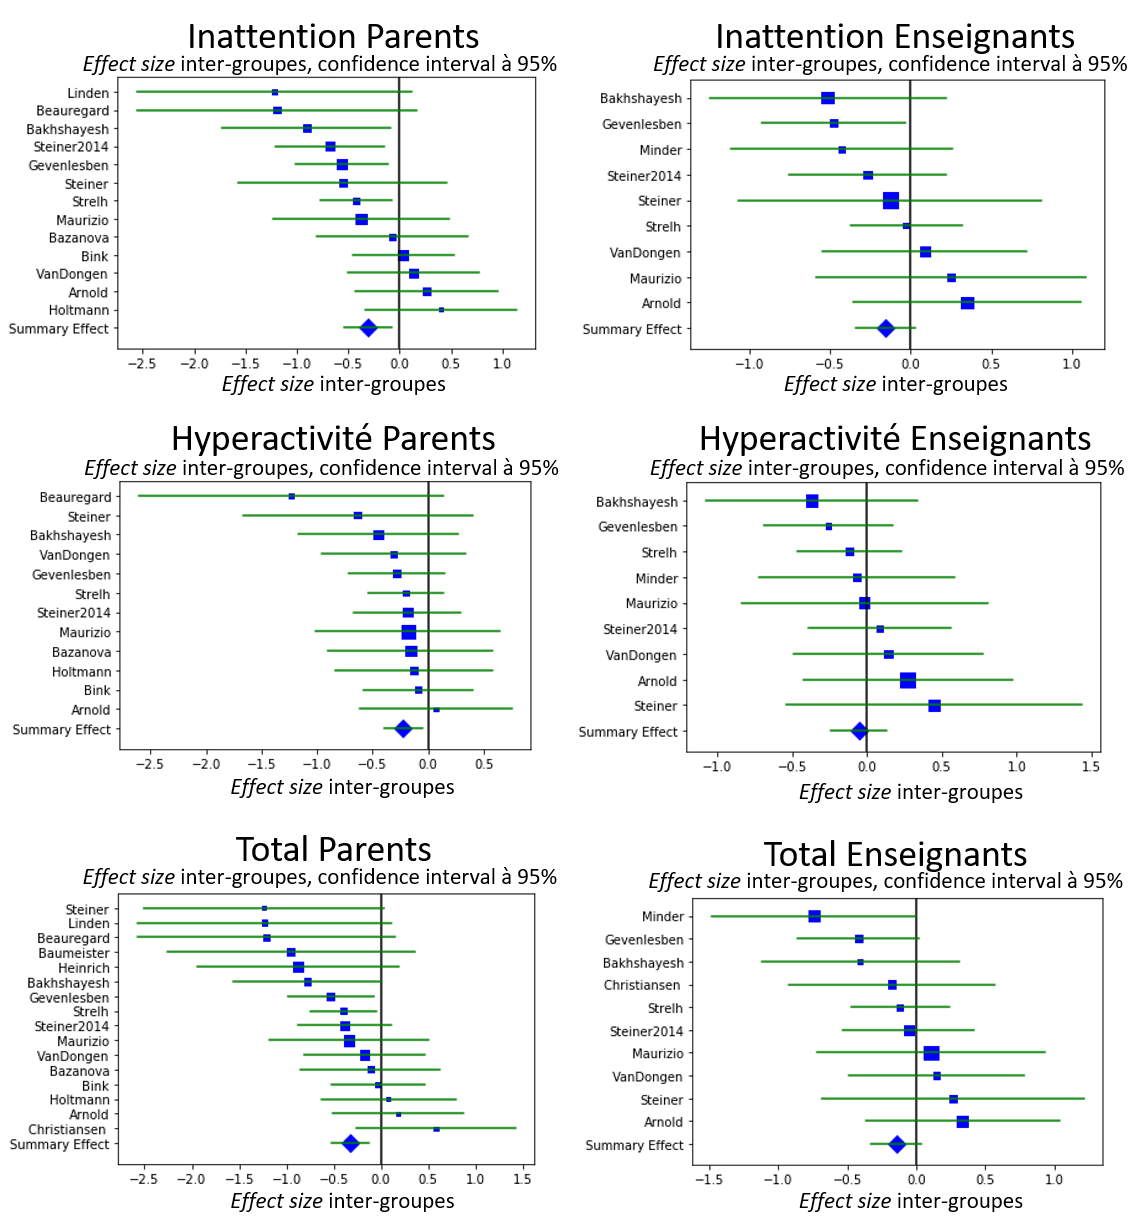
\includegraphics[width=1\linewidth]{figures/chapter-2/meta-analysis-forest-plots} 
  \caption{Forest plots des \gls{es}-inter-groupes (les carrés bleus) avec leur intervalle de confiance à 95\% (en vert) obtenus après la mise à jour de 
	\citet{Cortese2016}. Le losange bleu correspond à l'\gls{est}.
	Un \gls{es} négatif est en faveur du \gls{nfb}.}
  \label{Figure:meta_analysis_forest_plots}
\end{figure}

Afin de détecter un biais de publication parmi les études incluses, 2 \textit{funnel plot} basés sur les \gls{es}-inter-groupes calculés sur les évaluations
des symptômes totaux par les parents et les enseignants sont tracés à la Figure~\ref{Figure:meta_analysis_funnel_plots}. 

\begin{figure}[h!]
  \centering
	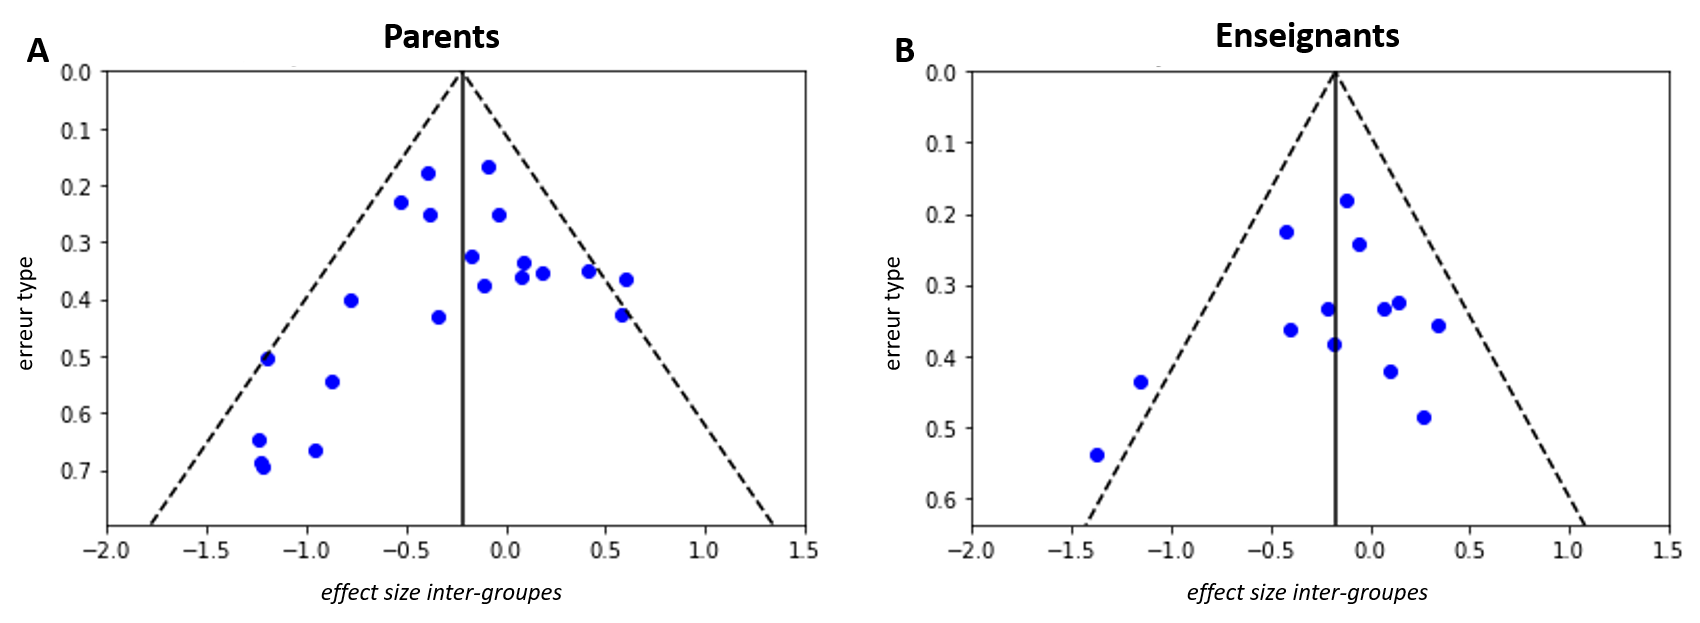
\includegraphics[width=1\linewidth]{figures/chapter-2/meta-analysis-funnel-plots} 
  \caption{Funnel plots obtenus pour les \gls{es}-inter-groupes calculés sur les évaluations des symptômes totaux par les parents (en \textbf{A)}) et 
	les enseignants (en \textbf{B)}) avec un intervalle de confiance à 95\%.}
  \label{Figure:meta_analysis_funnel_plots}
\end{figure}

Visuellement, alors que le \textit{funnel plot} correspondant aux \gls{est} des enseignants semble symétrique, celui des parents parait asymétrique, 
toutefois pour plus de précision le test d'Egger a également été utilisé pour déterminer statistiquement si un biais s'est glissé dans l'analyse :
\begin{description}
\item[pour les parents :] contrairement à ce qui est observé, le \textit{funnel plot} n'est pas asymétrique selon le test d'Egger, l'intercept ne diffère pas 
significativement de 0 (p-value = 0.281). \citet{Cortese2016}
avait également trouvé ce résultat (p-value = 0.133),
\item[pour les enseignants :]  le \textit{funnel plot} n'est pas non plus asymétrique (p-value = 0.235) alors que \citet{Cortese2016} avait trouvé un biais
(p-value = 0.042).
\end{description}

\subsubsection{Résultats sur les sous-groupes}

L'efficacité du \gls{nfb} a également été évaluée au sein de sous populations \citep{Cortese2016} avec les choix définis en \ref{replication} et en ajoutant
les nouvelles études. 

La première sous population étudiée correspond aux sujets ayant suivi un entraînement par \gls{nfb} \emph{standard}, c'est à dire répondant aux critères établis
par \citet{Arns2014} :
\begin{itemize}
\item le protocole de \gls{nfb} utilisé a fait l'objet de plusieurs études cliniques (diminution du \gls{tbr}, augmentation du \gls{smr} et \gls{scp}),
\item une phase de transfert doit être proposée durant l'entraînement pour aider la transposition dans la vie de tous les jours,
\item le lieu où sont effectuées les sessions doit être précisé,
\item le traitement par \gls{nfb} doit satisfaire les critères de la théorie de l'apprentissage, c'est à dire ne pas utiliser de seuil de récompense automatique.
\end{itemize}

Parmi les 13 études initialement incluses, \citet{Cortese2016} en a identifié 7 mettant en place un protocole de \gls{nfb} standard \citep{Bakhshayesh2011,
Christiansen2014, Gevensleben2009, Beauregard2006, Holtmann2009, Heinrich2004, Linden1996}. 
Les \gls{est} calculés sont tous significativement en faveur du \gls{nfb}, sauf pour la composante hyperactivité évaluée par les enseignants (p-value = 0.11). 
L'ajout des 2 études correspondant à cette définition \citep{Strehl2017, Baumeister2016} conduit aux mêmes résultats. 

La deuxième sous population étudiée comprend les sujets ne prenant aucun traitement médicamenteux durant le traitement par \gls{nfb}. A l'origine, 7 études
sont incluses dans cette analyse \citep{Beauregard2006, Gevensleben2009, Bakhshayesh2011, Arnold2014, Linden1996, Christiansen2014, Maurizio2014} et la 
mise à jour conduit à l'ajout de \citep{Bazanova2018}. Pour ce sous-groupe, seul l'\gls{est} de la composante inattention évaluée par les parents est significatif
(p-value = 0.017). En effet, les différences dans les valeurs à post-test de \citet{Arnold2014} et l'inclusion de \citet{Bazanova2018} a conduit à la perte de 
significativité de l'\gls{est} de la composante hyperactivité évaluée par les parents (p-value = 0.062) par rapport au résultat de \citet{Cortese2016} (p-value 
= 0.016).

\section{Discussion} 

Les méta-analyses doivent être menées rigoureusement, ainsi pour guider les auteurs des recommandations existent comme celles de PRISMA \citep{Moher2009}.
La réplication et la mise à jour présentées ici remplissent la majorité des points de la checklist, sauf notamment l'évaluation du risque de biais dans chaque étude.
 
Le travail décrit précédemment a pour but d'explorer l'impact de certains choix de \citet{Cortese2016} qui ont été débattus dans la communauté scientifique 
\citep{Micoulaud2016}. Nous résumons ici la liste des changements, leur justification et leurs conséquences sur les résultats. Par ailleurs, l'importance de mettre 
à jour ces analyses est soulignée.

\subsection{Discussion sur les résultats obtenus} \label{replication_and_update}

Les résultats obtenus suite à la réplication et à la mise à jour de \citet{Cortese2016} sont analysés et mis en perspective avec la littérature existante ici.

\subsubsection{Réplication}

Un des choix qui a été fait ici est d'utiliser la Conners-3 Teachers \citep{Conners2008} plutôt que la BOSS Classroom \citep{Shapiro2010} 
pour calculer les \gls{es}-inter-groupes obtenus par les évaluations des enseignants du fait de son utilisation plus commune \citep{Christiansen2014, Bluschke2016}.
Toutefois, l'utilisation de l'une ou l'autre de ces échelles ne change pas la significativité des \gls{est} calculés pour les enseignants. 

La seconde différence entre \citep{Cortese2016} et la réplication effectuée ici est que le calcul des \gls{es}-inter-groupes de \citet{Arnold2014} se base 
sur les valeurs à post-test obtenues après 40 sessions de \gls{nfb} au lieu de valeurs temporaires obtenues après 12 sessions. Des études montrent
que le nombre de sessions est corrélé positivement avec les changements observés sur l'\gls{eeg} \citep{Vernon2004}, ainsi un faible nombre de sessions mènerait
à des \gls{es}-inter-groupes plus petits. Or, ici les \gls{es}-inter-groupes calculés après la réalisation de toutes les sessions sont plus faibles que ceux 
obtenus après 12 sessions. Toutefois, ces différences ne changent pas la significativité des \gls{est}. 

Par conséquent, bien que ces points aient été débattus, leur impact sur les conclusions de la méta-analyse sont minimes et ne changent la significativité
d'aucun \gls{est}. 

\subsubsection{Mise à jour}

L'ajout des trois nouvelles études \citep{Baumeister2016, Strehl2017, Bazanova2018} confirment les résultats obtenus par \citep{Cortese2016}. En effet,
la significativité des \gls{est} n'est pas modifiée : ils restent significatifs pour les parents mais non significatifs pour les enseignants. 

Ces trois nouvelles études apportent plus de puissance statistique aux résultats, notamment pour l'analyse des sous-groupes menée par \citet{Cortese2016}.
En effet, pour la sous population suivant un protocole \gls{nfb} standard \citep{Arns2014}, \citet{Cortese2016} avait noté que les \gls{pblind} observaient
une différence statistiquement significative entre le \gls{nfb} et les groupes contrôles en faveur du \gls{nfb}. Cette tendance a été confirmée avec l'ajout 
de \citet{Baumeister2016} et \citet{Strehl2017} qui apportent 73 sujets supplémentaires, ce qui suggère une relation positive entre les caractéristiques des protocoles standards
et la performance du \gls{nfb}. 

\subsection{Hétérogénéité des études} 

Même si les méta-analyses regroupent les études répondant toutes aux critères d'inclusion comme, par exemple, ceux énoncés à \ref{selection_studies}, 
elles diffèrent tout de même sur de nombreux points, limitant la fiabilité de leurs résultats comme le souligne \citep{Alkoby2017}. Afin de pallier 
cette hétérogénéité, l'analyse peut cibler une population plus précise, comme ce qui a été effectué lors de l'analyse
des sous populations. Cependant, ce genre de restriction souffre d'une puissance statistique plus faible et regroupe encore des études fortement hétérogènes.
En effet, même si seuls les protocoles \gls{scp}, \gls{tbr} et \gls{smr} sont utilisés, ils restent intrinsèquement différents et il est probable que leur
efficacité ne soit pas la même. 

Par ailleurs, le matériel d'acquisition utilisé, ainsi que le traitement du signal varient d'une étude à l'autre, or ces points sont sans doute centraux 
dans la performance du traitement. 

De plus, aucun consensus n'existe quant au nombre de sessions ou à la durée du traitement, ainsi ces choix sont très variables d'une étude à l'autre et peu
souvent questionnés, bien qu'ils soient centraux dans la théorie de l'apprentissage.

\subsection{Importance de la mise à jour des méta-analyses}

Afin d'éviter de tomber dans le \textit{p-hacking}, il est important de ne pas arrêter la collecte de données et donc de figer les résultats une fois 
que la p-value de l'\gls{est} passe sous le seuil de signicativité de 0.05 \citep{Head2015, Coffman2015}. En effet, l'arrêt prématuré des résultats peut
générer un biais : par exemple la p-value peut être significative à un instant t avec un certain nombre de sujets inclus, puis perdre sa significativité à
t $+$ 1 et ne plus la retrouver. Mettre à jour les résultats même dans le cas où la p-value est significative est donc préférable, les résultats étant
davantage fiables une fois que la p-value converge. Ces deux configurations sont représentées à la Figure~\ref{Figure:meta-analysis-evolution-p-value-examples}

\begin{figure}[h!]
  \centering
	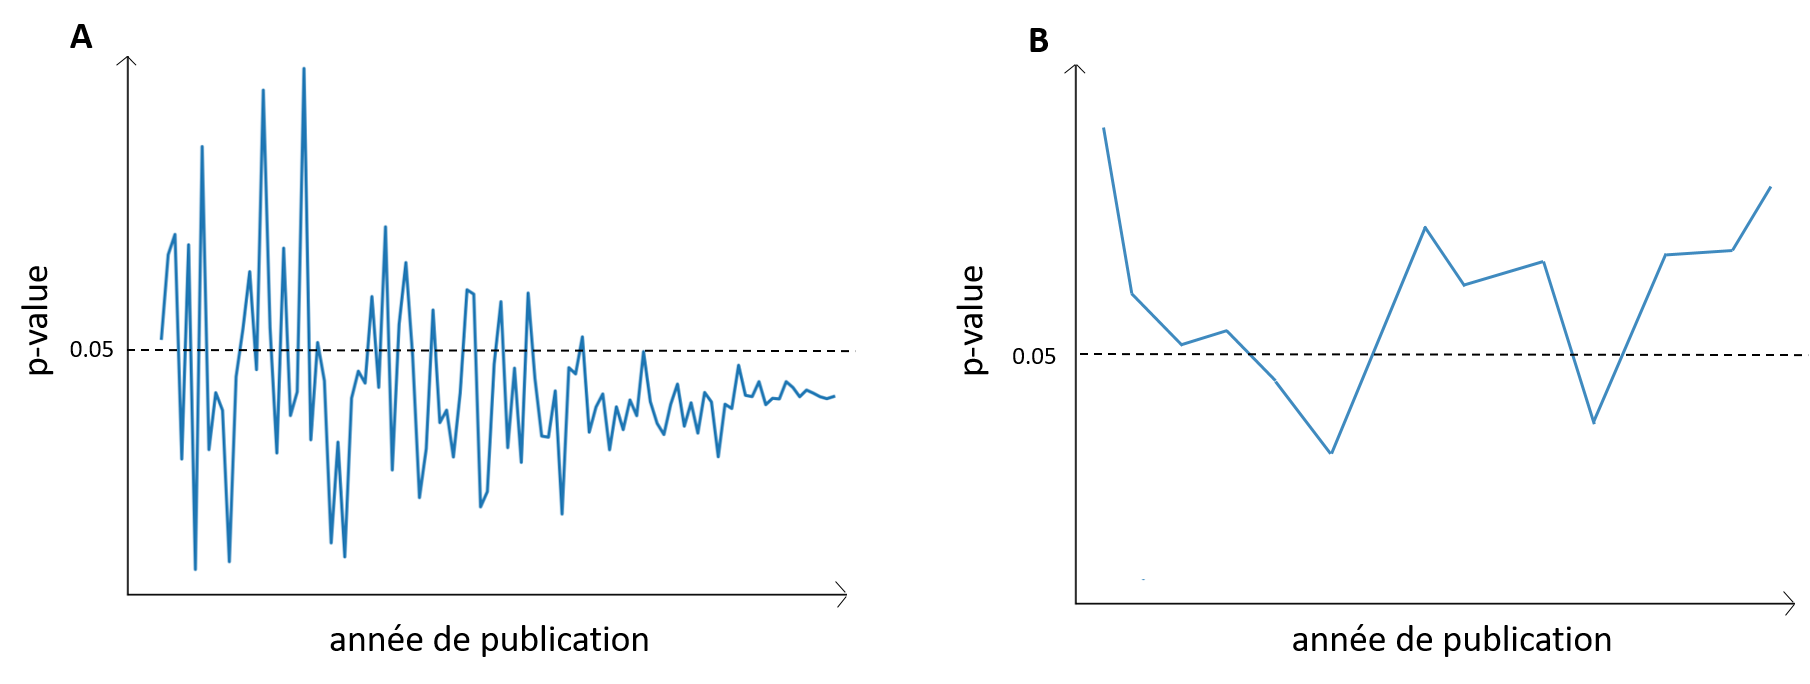
\includegraphics[width=1\linewidth]{figures/chapter-2/meta-analysis-evolution-p-value-examples} 
  \caption{Exemples d'évolution de la p-value des \gls{est} au fur et à mesure de l'ajout des études sur des fausses données. 
	En \textbf{A}, la p-value converge suite à l'ajout de nouvelles études ; en \textbf{B} l'évolution de la p-value n'est pas stable. 
	Le seuil de significativité à 0.05 est représenté en pointillés noirs.}
  \label{Figure:meta-analysis-evolution-p-value-examples}
\end{figure}

Les résultats d'une méta-analyse peuvent donc souffrir de l'arrêt prématuré des résultats lorsque la p-value de l'\gls{est} n'est pas stable, comme 
illustré à la Figure~\ref{Figure:meta_analysis_evolution_pvalue} où l'évolution des p-values des \gls{est} de la composante totale en fonction des études 
incluses au fur et à mesure selon leur année de publication est tracée. Les écarts types mobiles des p-values sont calculés en prenant les trois plus
plus récentes p-values (dont celle pour laquelle on calcule cet écart type). Une approche mobile est préférée ici à une approche fixe qui prend en 
compte l'ensemble des p-values passées qui sont obtenues sur un plus petit nombre d'études.

\begin{figure}[h!]
  \centering
	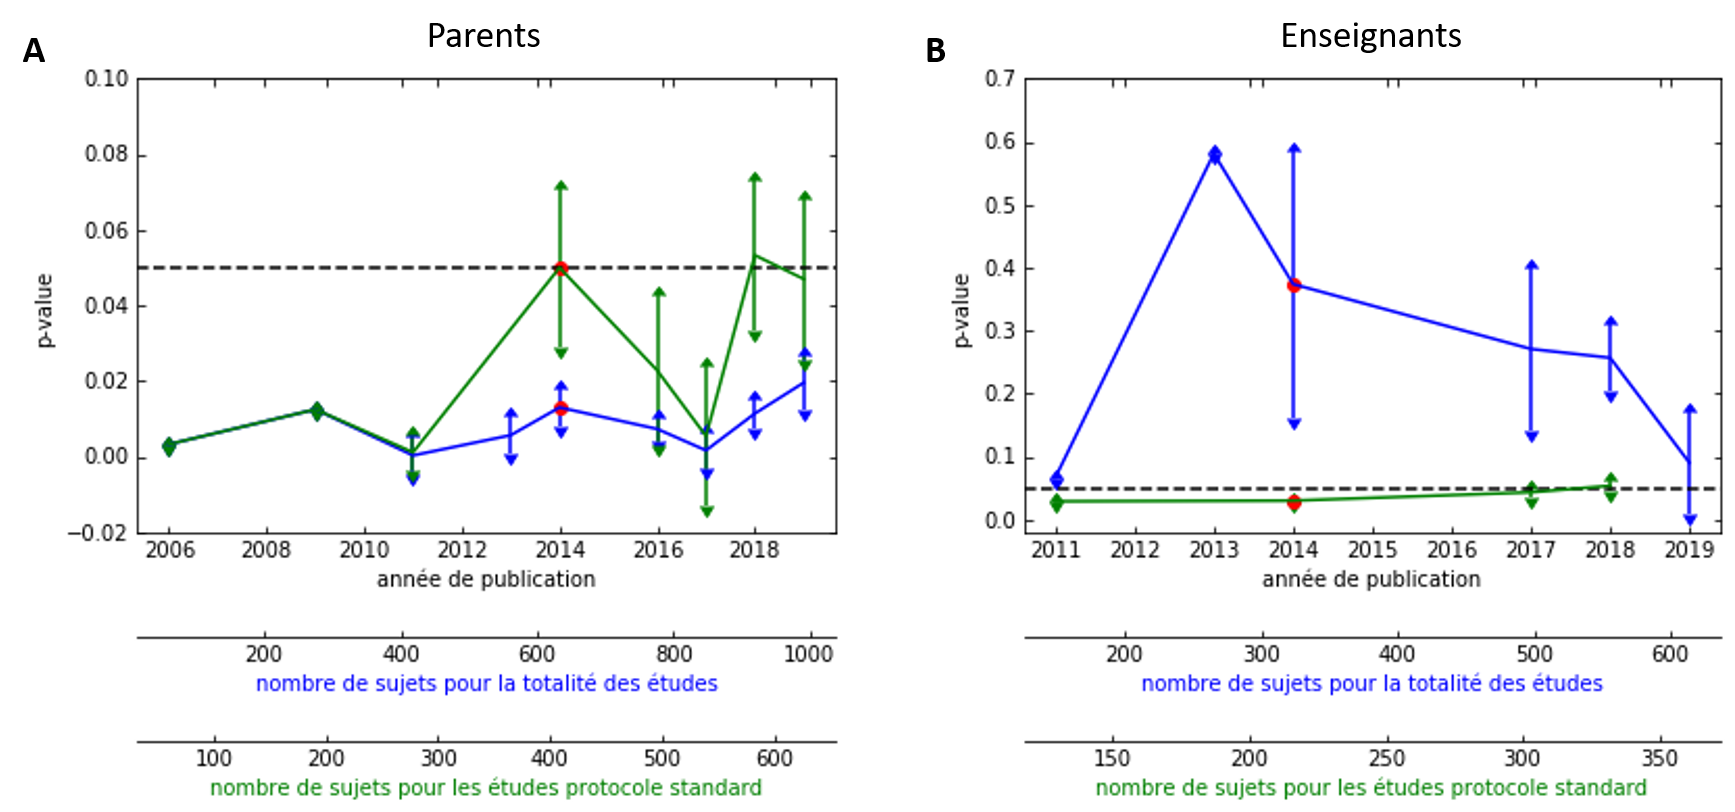
\includegraphics[width=1\linewidth]{figures/chapter-2/meta-analysis-evolution-p-value} 
  \caption{Evolution de la p-value des \gls{est} au fur et à mesure de l'ajout des études pour les évaluations des 
	parents en \textbf{A} et des enseignants en \textbf{B} sur la composante totale.
	La courbe verte correspond aux études incluses dans la sous population du protocole \gls{nfb} standard et la courbe bleue à la totalité des études.
	Le nombre de sujets inclus dans ces deux groupes en fonction des années de publications est donné. Le point rouge correspond aux résultats de \citet{Cortese2016}.
	Les écarts types mobiles (calculés sur les trois dernières p-values) sont représentés. 
	Le seuil de significativité à 0.05 est représenté en pointillés noirs.}
  \label{Figure:meta_analysis_evolution_pvalue}
\end{figure}

A première vue, la plus forte fluctuation correspond à la p-value des \gls{est} obtenues sur la totalité des études pour les évaluations des enseignants 
(en bleu sur le graphique \textbf{B} de la Figure~\ref{Figure:meta_analysis_evolution_pvalue}). En effet, en 2013 la p-value atteint un pic à 0.6, cependant 
depuis 2014 elle diminue de façon stable (sauf entre 2018 et 2019) et tend de plus en plus vers la significativité, sans converger pour le moment, ce qui 
laisse penser que plus d'études sont nécessaires afin de vraiment pouvoir conclure quant à l'efficacité du \gls{nfb} selon les enseignants. L'évolution
de la p-value dans le sous groupe des protocoles standards (en vert sur le graphique \textbf{B}) est stable, comme le montrent notamment les écarts types mobiles. 

En ce qui concerne les p-values des \gls{est} obtenus grâce aux évaluations des parents représentées sur le graphique \textbf{A} de la 
Figure~\ref{Figure:meta_analysis_evolution_pvalue}, elles varient mais ne dépassent pas le seuil de significativité (sauf légèrement
en 2018). L'évolution des p-values pour le groupe du protocole \gls{nfb} standard (en vert sur le graphique \textbf{A}) fluctue
depuis 2011, ce qui cause une augmentation de l'écart type mobile : un plus grand nombre d'études à inclure dans ce groupe serait bienvenu afin 
de stabiliser la p-value. A l'inverse, l'évolution de la p-value calculée pour la totalité des études (en bleu sur le graphique \textbf{A}) est assez stable
et présente des déviations standards mobiles plus faibles. Cette évolution est la plus stable du fait du nombre d'études incluses (et donc de sujets inclus)
qui le est le plus important entre les quatre groupes étudiés ici. 

Ainsi, depuis la méta-analyse de \citet{Cortese2016}, dont les résultats sont représentés par un point rouge sur chaque courbe de la 
Figure~\ref{Figure:meta_analysis_evolution_pvalue}, les p-values ont fluctué même si aucun changement de significtaivité n'est observé. 
Cette absence de stabilité appelle à de nouvelles mises à jour : une a été effectuée et a été décrite en \ref{selection_studies} \citep{Bussalb2019clinical},
cependant depuis de nouvellles études ont été publiées. 

Ainsi, une nouvelle recherche sur PubMed a été lancée le 2 septembre 2019 en suivant les mêmes étapes que présentées en \ref{selection_studies}, le détail
des études identifiées est donné à la Table~\ref{Table:table_meta_review_update_september_2019}.


\begin{table}[h!]
  \centering
  \caption{Détails des études satisfaisant les critères d'inclusion de \citep{Cortese2016} après la recherche PubMed du 2 septembre 2019.}
  \begin{tabular}{ccc}
\toprule
Articles & \shortstack{ Nombre de \\ sujets} & Résultats disponibles \\
\toprule
\multirow{2}{*}{ \citet{Aggensteiner2019} } & $75$ \gls{nfb} & parents : total et inattention \\
                                          & $69$ contrôles & enseignants : / \\		
\midrule
\multirow{2}{*}{ \citet{Minder2018} } &  $19$ \gls{nfb} & parents : total, inattention, hyperactivité \\
                                      & $19$ contrôles & enseignants : total, inattention, hyperactivité \\ 
\midrule
\multirow{2}{*}{ \citet{Moreno2019} } & $19$ \gls{nfb} & parents : total \\
                                      & $19$ contrôles & enseignants : total \\
\midrule
\multirow{2}{*}{ \citet{Shereena2019} } & $15$ \gls{nfb} & parents : total, inattention, hyperactivité \\
                                      & $19$ contrôles & enseignants : total, inattention, hyperactivité \\
\bottomrule
\end{tabular}

  \label{Table:table_meta_review_update_september_2019}
\end{table} 

Avec cette mise à jour, la méta-analyse comprend désormais 20 articles : les résultats sont globalement les mêmes qu'après la première mise à jour, la seule
différence importante est la perte de la significativité de l'\gls{est} pour la composante hyperactivité évaluée par les parents (p-value = 0.069).
Les \gls{est} évalués par les enseignants sont, quant à eux, toujours non significatifs (p-value pour la composante totale =  0.09).

En ce qui concerne les résultats dans les sous-groupes :
\begin{description}
\item[protocole standard :] 2 études ont été ajoutées \citep{Aggensteiner2019, Minder2018} et rendent tous les \gls{est} initialement significatifs 
non significatifs ; désormais seul l'\gls{est} de la composante totale évaluée par les parents est encore significatif (p-value = 0.047). 
L'\gls{est} calculé pour la composante totale évaluée par les enseignants est limite significatif (p-value = 0.053),
\item [pas de traitement médicamenteux en simultané :] seule une étude a été ajoutée \citep{Moreno2019} et aucune modification de significativité
n'est observée.
\end{description}

Ainsi, ces résultats démontrent que les résultats varient encore avec l'inclusion de nouvelles études, ce qui valide ce qui a été dit précédemment
sur l'importance de mettre à jour les méta-analyses tant que les résultats fluctuent encore. 

Cette approche qui consiste à affiner les résultats à l'aide de nouvelles observations est l'une des bases de l'inférence bayésienne.

\section{Conclusion}

Le but de ce travail était d'explorer les choix effectués par \citet{Cortese2016} dans leur méta-analyse et de rendre cette méthode plus transparente grâce
à l'élaboration d'un package Python. Il se trouve que les choix effectués par \citet{Cortese2016} n'influencent pas les conclusions finales. Ces conclusions
restent par ailleurs inchangées après la mise à jour de cette méta-analyse. Mettre à jour ce type d'analyse est nécessaire pour obtenir des résultats de plus
en plus fiables du fait du nombre toujours croissant d'études sur le \gls{nfb} appliqué au \gls{tdah}. 

Les méta-analyses étudiant l'effet du \gls{nfb} appliqué aux enfants \gls{tdah} utilisent des évaluations cliniques données par les parents et les enseignants.
Ces évaluations sont donc subjectives et, de plus, ne rendent peut-être pas compte de l'effet spécifique du \gls{nfb}. Pour capturer cet effet, il faut
s'intéresser aux neuromarqueurs et examiner la corrélation entre les changements dans le profil \gls{eeg} des sujets et les évaluations comportementales.

Toutefois, les résultats des méta-analyses donnent une idée de l'efficacité du traitement étudié, même s'il faut garder à l'esprit que les études incluses
diffèrent sur différents points, ce qui est notamment vrai pour le \gls{nfb}. Ces points ont sans doute une influence sur l'efficacité du \gls{nfb}, ainsi nous 
proposons dans le chapitre suivant de tirer avantage de cette hétérogénéité pour tenter de mettre en évidence les facteurs techniques et/ou cliniques qui
pourraient avoir une influence sur la performance du \gls{nfb}.

% trouver de la biblio
  